%%
%% This is file `sample-manuscript.tex',
%% generated with the docstrip utility.
%%
%% The original source files were:
%%
%% samples.dtx  (with options: `manuscript')
%% 
%% IMPORTANT NOTICE:
%% 
%% For the copyright see the source file.
%% 
%% Any modified versions of this file must be renamed
%% with new filenames distinct from sample-manuscript.tex.
%% 
%% For distribution of the original source see the terms
%% for copying and modification in the file samples.dtx.
%% 
%% This generated file may be distributed as long as the
%% original source files, as listed above, are part of the
%% same distribution. (The sources need not necessarily be
%% in the same archive or directory.)
%%
%% The first command in your LaTeX source must be the \documentclass command.
%%%% Small single column format, used for CIE, CSUR, DTRAP, JACM, JDIQ, JEA, JERIC, JETC, PACMCGIT, TAAS, TACCESS, TACO, TALG, TALLIP (formerly TALIP), TCPS, TDSCI, TEAC, TECS, TELO, THRI, TIIS, TIOT, TISSEC, TIST, TKDD, TMIS, TOCE, TOCHI, TOCL, TOCS, TOCT, TODAES, TODS, TOIS, TOIT, TOMACS, TOMM (formerly TOMCCAP), TOMPECS, TOMS, TOPC, TOPLAS, TOPS, TOS, TOSEM, TOSN, TQC, TRETS, TSAS, TSC, TSLP, TWEB.
% \documentclass[acmsmall]{acmart}

%%%% Large single column format, used for IMWUT, JOCCH, PACMPL, POMACS, TAP, PACMHCI
% \documentclass[acmlarge,screen]{acmart}

%%%% Large double column format, used for TOG
% \documentclass[acmtog, authorversion]{acmart}

%%%% Generic manuscript mode, required for submission
%%%% and peer review
%\documentclass[manuscript,screen,review]{acmart}
\documentclass[sigconf,review]{acmart}


%% Fonts used in the template cannot be substituted; margin 
%% adjustments are not allowed.
%%
%% \BibTeX command to typeset BibTeX logo in the docs
\AtBeginDocument{% 
 \providecommand\BibTeX{{%
   \normalfont B\kern-0.5em{\scshape i\kern-0.25em b}\kern-0.8em\TeX}}}
    
  %  \AtBeginDocument{\renewcommand*{\thesubfigure}{\alphalph{\value{subfigure}}}}

%% Rights management information.  This information is sent to you
%% when you complete the rights form.  These commands have SAMPLE
%% values in them; it is your responsibility as an author to replace
%% the commands and values with those provided to you when you
%% complete the rights form.


\setcopyright{none} % remove permission section
\settopmatter{printacmref=false} % remove ACM reference format
\renewcommand\footnotetextcopyrightpermission[1]{} % removes footnote with conference information in first column
\pagestyle{plain}
%\setcopyright{acmcopyright}
%\copyrightyear{2022}
%\acmYear{2022}
%\acmDOI{00.0000/0000000.0000000}

%% These commands are for a PROCEEDINGS abstract or paper.
%\acmConference[Woodstock '18]{Woodstock '18: ACM Symposium on Neural Gaze Detection}{June 03--05, 2018}{Woodstock, NY}
\acmConference[SSW 625]{SSW 625: Artificial Intelligence for Software Engineering}{November 2026}{Stevens Institute of Technology, Hoboken, NJ, USA}
\acmBooktitle{SSW 625: Artificial Intelligence for Software Engineering, Stevens Institute of Technology, November 2026}

\usepackage{xspace}
\newcommand{\ie}{\textit{i.e.}}
\newcommand{\eg}{\textit{e.g.}}
\newcommand{\etal}{\textit{et al. \xspace}}
%\usepackage{array}
%\newcolumntype{L}{>{\arraybackslash}m{8cm}}
%%%%% Long text wrap %%%%%
\usepackage{array}
\newcolumntype{L}{>{\arraybackslash}m{16cm}}
%\newcolumntype{L}[1]{>{\raggedright\let\newline\\arraybackslash\hspace{0pt}}m{#1}}
\newcolumntype{C}[1]{>{\centering\let\newline\\arraybackslash\hspace{0pt}}m{#1}}
\newcolumntype{R}[1]{>{\raggedleft\let\newline\\arraybackslash\hspace{0pt}}m{#1}}
%%%%% Long text wrap %%%%%
%\usepackage{adjustbox}
%\usepackage{subcaption}
%\usepackage{textcomp}
%\usepackage{pgfplots}
%\usepackage{soul}
%\usepackage{booktabs}
%\usepackage{multirow}
%\usepackage{float}
%\usepackage{url}
\usepackage{tcolorbox}
\usepackage{graphicx}
%\usepackage{textcomp}
\usepackage{xcolor}
%\usepackage{url}
%\usepackage{tabularx} 
%\usepackage{balance}
\usepackage{stfloats}
%\usepackage{fullpage}
\usepackage[justification=centering]{caption}
\usepackage{lineno}
\usepackage[title]{appendix}
\usepackage{dirtytalk}
\usepackage{amsmath}
%\usepackage{tikz}
\usepackage{pgfplots, pgfplotstable}
%\usetikzlibrary{tikzmark}
\usetikzlibrary{patterns}



%%%%%
%-----------------------
%\usepackage[utf8]{inputenc}
\usepackage[english]{babel}
%\usepackage{amssymb}
\usepackage{textcomp}
%\usepackage{indentfirst}
%\setcounter{tocdepth}{3}
\usepackage{mathtools}
%\usepackage[usestackEOL]{stackengine}
%\usepackage{amsmath}
\usepackage{ltxtable}
\usepackage{algorithm}
\usepackage{algpseudocode}
\usepackage{textcomp}
%\usepackage{mathpazo}
%\usepackage{tgpagella}
%-----------------------

\usepackage{tcolorbox}

%\usepackage[dvipsnames]{xcolor}
\usepackage{pgf-pie}
%\usepackage{pgfplots}
%\pgfplotsset{compat=1.14}
%%%%%%%%%%%%%%%%%%%%%%%%%%%%%%%%%%%%%%%%%%%%%%%%%%%
\definecolor{wedge1}{RGB}{ 190  30  46}
\definecolor{wedge2}{RGB}{ 240  65  54}
\definecolor{wedge3}{RGB}{ 241  90  43}
\definecolor{wedge4}{RGB}{ 247 148  30}
\definecolor{wedge5}{RGB}{  43  56 144}
\definecolor{wedge6}{RGB}{  28 117 188}
\definecolor{wedge7}{RGB}{  40 170 225}
\definecolor{wedge8}{RGB}{ 119 179 225}
\definecolor{wedge9}{RGB}{ 181 212 239}
\definecolor{wedge10}{RGB}{  0 104  56}
\definecolor{wedge11}{RGB}{  0 148  69}
\definecolor{wedge12}{RGB}{ 57 181  74}
\definecolor{wedge13}{RGB}{141 199  63}
\definecolor{wedge14}{RGB}{215 244  34}
\definecolor{wedge15}{RGB}{249 237  50}
\definecolor{wedge16}{RGB}{248 241 148}
\definecolor{wedge17}{RGB}{242 245 205}
\definecolor{wedge18}{RGB}{123  82  49}
\definecolor{wedge19}{RGB}{104  73 158}
\definecolor{wedge20}{RGB}{102  45 145}
\definecolor{wedge21}{RGB}{148 149 151}
\definecolor{wedge22}{RGB}{ 204 50 153}
\definecolor{wedge23}{RGB}{ 79 47 79}
\definecolor{wedge24}{RGB}{ 173 234 234}
\definecolor{wedge25}{RGB}{ 216 191 216}
\definecolor{wedge26}{RGB}{  43  56 144}
\definecolor{wedge27}{RGB}{  40 170 225}
\definecolor{wedge28}{RGB}{ 119 179 225}
\definecolor{wedge29}{RGB}{ 181 212 239}
\definecolor{wedge30}{RGB}{  0 104  56}
\definecolor{wedge31}{RGB}{  0 148  69}
\definecolor{wedge32}{RGB}{ 57 181  74}

\usetikzlibrary{chains}
%%%%%%%%%%%%%%%%%%%%%%%%%%%%%%%%%%%%%%


\def\groupTotals{{1,4,5,8,1,2}}
\pgfmathsetmacro\startAngle{90-3.6/2}
\pgfmathsetmacro\radius{+5}
\pgfmathsetmacro\maxLeg{+12}
\pgfmathsetmacro\legBound{+60}
\pgfmathsetmacro\legSpacing{2*\legBound/(\maxLeg-1)}
%%%%%%%%%%%%%%%%%%%%%%%%%%%%%%%%%%%%%%

%%%%%%%%%%%%%%%%%%%%%%%%%%%%%%%%%%%%%
\usepackage{verbatim}
%\usepackage{pgfplots, pgfplotstable}
%\pgfplotsset{width=7cm,compat=1.8}
%\pgfplotsset{width=7cm,compat=1.8,tick label style={font=\small}}
\pgfplotsset{compat=1.14}
\usetikzlibrary{patterns,}

\usepackage{graphicx}
\usepackage{tabularx,booktabs}
\usepackage{array}
\usepackage{bbding}
\usepackage{pifont}
\usepackage{wasysym}
%\usepackage{amssymb}
\usepackage{caption}
\usepackage{dirtytalk}
%\usepackage[showframe]{geometry}
%\usepackage{subfigure}
\usepackage{subcaption}
%\usepackage{amsmath} % Star
%\usepackage[table]{xcolor}
\usepackage{tabularx}
%\usepackage{pgfplots}
%\usepackage{pgf-pie}
%\usepackage{verbatim}
%\usepackage{pgfplotstable}
\usepackage{sfmath}
\usepackage{array, booktabs, makecell}
\usepackage{color}
%\usepackage[dvipsnames]{xcolor}
\usepackage{csquotes}
\usepackage{url}
\usepackage{comment}
\usepackage{tikz}
\usepackage{balance}
\usepackage{listings}
\usepackage{booktabs} % used for \toprule in tables
%\usepackage{cite}
\usepackage{soul} % highlighting
\urlstyle{same} %% footnote fonts
\usetikzlibrary{fit} %% Used for putting dotted box in image
%\usepackage[margin=2cm]{geometry}
\usetikzlibrary{positioning}
\usetikzlibrary{arrows}
\usetikzlibrary{shapes.multipart}
%\usepackage{caption}
%\usepackage{graphicx}
\usepackage{adjustbox}
%\usepackage{tablefootnote}
\usepackage{float}
\usepackage{rotating}
\usepackage{nth}
\DeclareCaptionType{TextBox}
\usepackage{pstricks}
%%%%%%%%%%%%%%%%%%%%%%%%%%%%%%%%%%%%%%%%%%%%%%%%%%%%%%%%
\usepackage{placeins}
\usepackage{afterpage}
\usepackage{multirow} 
\usepackage{textcomp}
\usepackage{multicol}
\usepackage{varwidth} % Double column tables
\usepackage{makecell}

%%%%%

%\usepackage{subfigure}
\newcommand{\eman}[1]{\textcolor{violet}{{\it [Eman says: #1]}}}

\lstset{
  basicstyle=\ttfamily\small,
  breaklines=true,
  breakatwhitespace=false,
  postbreak=\mbox{\textcolor{gray}{$\hookrightarrow$}\space},
  columns=fullflexible,
  keepspaces=true,
  frame=single,
  numbers=left,
  numberstyle=\tiny
}


%%
%% Submission ID.
%% Use this when submitting an article to a sponsored event. You'll
%% receive a unique submission ID from the organizers
%% of the event, and this ID should be used as the parameter to this command.
%%\acmSubmissionID{123-A56-BU3}

%%
%% The majority of ACM publications use numbered citations and
%% references.  The command \citestyle{authoryear} switches to the
%% "author year" style.
%%
%% If you are preparing content for an event
%% sponsored by ACM SIGGRAPH, you must use the "author year" style of
%% citations and references.
%% Uncommenting
%% the next command will enable that style.
%%\citestyle{acmauthoryear}

%%
%% end of the preamble, start of the body of the document source.
\begin{document}

%%
%% The "title" command has an optional parameter,
%% allowing the author to define a "short title" to be used in page headers.
\title{Modern Supply Chain Attacks: An Issue of Trust in AI Agent Ecosystems}


\author{Abdul Rahim Shahad}
%\authornote{Both authors contributed equally to this research.}
\email{ashahad@stevens.edu}
\affiliation{%
  \institution{Stevens Institute of Technology}
  %\streetaddress{P.O. Box 1212}
  \city{Hoboken}
  \state{New Jersey}
  \country{USA}
  %\postcode{43017-6221}
}

\author{Irakli Dokhnadze}
%\authornote{Both authors contributed equally to this research.}
\email{idokhnad@stevens.edu}
\affiliation{%
  \institution{Stevens Institute of Technology}
  %\streetaddress{P.O. Box 1212}
  \city{Hoboken}
  \state{New Jersey}
  \country{USA}}
  
\author{Abdul Karim Mohammed}
%\authornote{Both authors contributed equally to this research.}
\email{amohamme25@stevens.edu}
\affiliation{%
  \institution{Stevens Institute of Technology}
  %\streetaddress{P.O. Box 1212}
  \city{Hoboken}
  \state{New Jersey}
  \country{USA}}
  
\author{Victor Del Rio Foces}
%\authornote{Both authors contributed equally to this research.}
\email{vdelriof@stevens.edu}
\affiliation{%
  \institution{Stevens Institute of Technology}
  %\streetaddress{P.O. Box 1212}
  \city{Hoboken}
  \state{New Jersey}
  \country{USA}}
  

%%
%% The "author" command and its associated commands are used to define
%% the authors and their affiliations.
%% Of note is the shared affiliation of the first two authors, and the
%% "authornote" and "authornotemark" commands
%% used to denote shared contribution to the research.


%%
%% By default, the full list of authors will be used in the page
%% headers. Often, this list is too long, and will overlap
%% other information printed in the page headers. This command allows
%% the author to define a more concise list
%% of authors' names for this purpose.
%\renewcommand{\shortauthors}{Trovato and Tobin, et al.}

%%
%% The abstract is a short summary of the work to be presented in the
%% article.
\begin{abstract}
AI agent skills are made up of \texttt{SKILL.md} files that frequently travel around an ecosystem with no registry. The GitSkills dataset tracks a total of 3,797,117 skill files, 50.5\% of which are exact copies. This consequently results in an issue of trust, as malware disguised within a \texttt{SKILL.md} file can easily propagate to hundreds or thousands of AI agents. We study this on the GitSkills sample of 29,786 skill files (13,000 distinct contents). Among 205 near-duplicate pairs of reused skills, 6 pairs add command execution and 16 pairs add network access that the original does not have, and 2 of the 13,000 distinct skills bundle executable files.

The source code and analysis pipeline used in this study are available at \url{https://github.com/FrillySnake/ssw625_project}.
\end{abstract}


%%
%% The code below is generated by the tool at http://dl.acm.org/ccs.cfm.
%% Please copy and paste the code instead of the example below.
%%
\begin{CCSXML}
<ccs2012>
 <concept>
  <concept_id>10010520.10010553.10010562</concept_id>
  <concept_desc>Computer systems organization~Embedded systems</concept_desc>
  <concept_significance>500</concept_significance>
 </concept>
 <concept>
  <concept_id>10010520.10010575.10010755</concept_id>
  <concept_desc>Computer systems organization~Redundancy</concept_desc>
  <concept_significance>300</concept_significance>
 </concept>
 <concept>
  <concept_id>10010520.10010553.10010554</concept_id>
  <concept_desc>Computer systems organization~Robotics</concept_desc>
  <concept_significance>100</concept_significance>
 </concept>
 <concept>
  <concept_id>10003033.10003083.10003095</concept_id>
  <concept_desc>Networks~Network reliability</concept_desc>
  <concept_significance>100</concept_significance>
 </concept>
</ccs2012>
\end{CCSXML}

\ccsdesc[500]{Software Engineering~Software Testing, Quality Assurance, and Maintenance}
\ccsdesc[300]{Software Engineering}
%% \ccsdesc{Computer systems organization~Robotics}
%% \ccsdesc[100]{Networks~Network reliability}

%%
%% Keywords. The author(s) should pick words that accurately describe
%% the work being presented. Separate the keywords with commas.
\keywords{software quality, mining software repositories, agent skill, SKILL.md, copy-based reuse, content hash, near duplicate, supply-chain attack, command execution}

%% A "teaser" image appears between the author and affiliation
%% information and the body of the document, and typically spans the
%% page.

%%
%% This command processes the author and affiliation and title
%% information and builds the first part of the formatted document.
\maketitle

\section{Introduction}
\label{Section:Introduction}

Agent skills are folders containing a \texttt{SKILL.md} file. The file holds natural-language instructions that tell a language-model coding agent how to handle a class of tasks. It starts with YAML front matter, usually a name and description, followed by a Markdown body containing the instructions. A skill may also include executable scripts and reference documents.

Anthropic published this format as an open specification in October 2025. At runtime, the agent matches the current task against a skill’s description and decides whether to load it. No compiler or type checker verifies that decision. There is also no central registry or package manager for skills. Developers reuse them by copying folders between repositories, usually with no formal review. This matters because a skill can tell an agent to run shell commands, fetch remote resources, or execute a bundled script.

\section{Problem Statement}
\label{Section:Problem}
There are countless agent skills and \texttt{SKILL.md} files publicly available in GitHub repositories and dedicated hosting platforms like SkillsMP. A public dataset containing millions of such skill files revealed that, when grouping them by content hash, more than 50\% of the files were byte-by-byte copies of another file in the dataset [1]. This shows that copying is a major way skills spread. 

However, with copying comes the result of unintended consequences. Consider how it has been tried and tested that copying code, either from an AI agent like Claude or from an online platform like StackOverflow, can lead to disastrous effects, especially when programmers make little to no effort to understand and correct the code they are copying. Agent skills and \texttt{SKILL.md} files suffer from precisely the same issue.

Because all of these skills are available publicly, widely reused skills are frequently modified to introduce additional functionality and posted online to further propagate. In many cases, a free-flowing system like this is vitally beneficial to AI agent operators; it allows them to more easily search for the skills that most closely match their requirements without the inconvenience of creating one from scratch. In other cases, though, these modifications can be subtle and deliberately malicious. For example, a modified copy could add a shell command, a remote download, or a bundled executable. Every repository that later copies that version inherits the change without a registry warning or package-review step. This is the equivalent of a supply-chain attack in the AI agent skill ecosystem.

To address this issue, we make use of the public GitSkills dataset, in which Destefanis et al. collected 3,797,117 \texttt{SKILL.md} files from 282,200 public GitHub repositories [1]. Destefanis et al. have found, according to the dataset, that 50.5\% are exactly identical copies of another file found within the dataset, meaning that around 1.8 million AI agents in public GitHub projects make use of a \texttt{SKILL.md} file taken directly from another GitHub project. As a platform dedicated primarily to hosting open-source projects, GitHub implements no built-in registry or verification system and the burden of safety and security lies on the user who adopts a foreign project's code.

Searching for identical copies, however, does not fully resolve the issue; rather, this tends to work only for cleanup, after the consequences of a supply-chain attack have already been realized. In this paper, we instead propose a method through which users can comb through datasets, like GitSkills or other ones used for online platforms like SkillsMP, and identify files which are near-copies of other files. Most malicious changes or additions in an agent skill or \texttt{SKILL.md} file are deliberately small and tucked away, making them easy to miss. Using the GitSkills dataset, we will study divergence among copies of the most reused skills and identify near-duplicate variants of common templates, comparing each variant with its reference version. The comparison will look for newly added command execution, network access, or bundled executable files. The main result will be a measure of the prevalence of how often copied skills contain hidden divergence and what type of, if any, risky capability was introduced.

\section{Related Work}
\label{Section:RelatedWork}
Supply-chain attacks targeting \texttt{SKILL.md} file surfaces are not a new issue and date back to when the system was introduced in 2025, although it did not draw much attention until early 2026. In January and February of 2026 emerged the "ClawHavoc" incident, when the popular AI agent platform OpenClaw became the subject of widespread malware and infection. During the worst of the infection, five of the top seven most used skills on OpenClaw contained malware [2]. Of the 3,984 skills pulled from ClawHub and skills.sh, 534 contained a critical security issue [3]. These issues ranged from forbidden commands to leaked industry secrets. These malicious files disguised themselves as reputable and popular searches such as "Google", "Solana wallet tracker", and "Polymarket Trader" [2].

Even in ecosystems with stricter registries following the ClawHavoc incident, maliciously modified \texttt{SKILL.md} files can still spread easily. Embedding-based retrieval systems in many agent skill platforms, used for fetching relevant \texttt{SKILL.md} files to satisfy user requests, can be manipulated by simple text triggers appended to such files, allowing them to win over 86.14\% of other fetched files and appear among the top of search request lists far more often [4]. Likewise, operator negligence allows a majority of these files to spread and maintain relevance. Malicious skill files are chosen with a 77\% likelihood over other similar files mainly due to modified descriptions [4]. The registries and verification systems that make up these ecosystems are, too, at fault. In a scanning environment akin to that of ClawHub, semantic evasion tactics allow malicious skills to avoid being determined as such in anywhere from 36.5 to 100\% of cases [4].

While extensive work has gone forth to document cases of supply-chain attacks in AI agent skill ecosystems due to the lack or failures of verification and to establish \texttt{SKILL.md} files as a surface for such attacks, how these files are subtly adjusted to insert malicious behavior in real world cases is less explored. This paper aims to fill that gap by analyzing the GitSkills dataset as its core experiment.


\begin{table*}[htbp]
\centering
\caption{Characteristics of Existing Studies}
\label{tab:existing_studies}

\scriptsize
\setlength{\tabcolsep}{3pt}
\renewcommand{\arraystretch}{1.3}

\begin{tabularx}{\textwidth}{
    p{1.5cm}
    p{0.8cm}
    p{2.0cm}
    p{2.4cm}
    X
    p{2.0cm}
    p{2.0cm}
    p{2.0cm}
}
\toprule
\textbf{Study} &
\textbf{Year} &
\textbf{Manual/Automatic} &
\textbf{Classification Method} &
\textbf{Category} &
\textbf{Machine Learning} &
\textbf{Training Size} &
\textbf{Result} \\
\midrule

Beurer-Kellner et al. [3] &
2026 &
No/Yes &
\texttt{mcp-scan} &
\makecell[l]{Structural Analysis \\
Code Classification} & 
N/A & 
Top-100 skills.sh skills & 
\makecell[l]{90-100\% recall \\
0\% false positives} \\

\midrule

Saha et al. [4] &
2026 &
No/Yes &
N/A & 
\makecell[l]{Code Manipulation \\
Non-Functional Changes} & 
N/A & 
100 public ClawHub skills &
\makecell[l]{86.14\% more likely discovery \\
77\% more likely selection} \\

\midrule

This work &
2026 &
Yes/Yes & 
N/A &
\makecell[l]{Structural Analysis} &
N/A &
\makecell[l]{GitSkills sample \\ (29,786 skills; \\ 13,000 distinct contents)} &
\makecell[l]{6 of 205 pairs add \\ command execution \\ 16 of 205 add network \\ access \\ 2 of 13,000 skills \\ bundle executables} \\

\bottomrule
\end{tabularx}
\end{table*}


\section{Study Design}
\label{Section:Methodology}
\begin{figure*}[t]
    \centering
    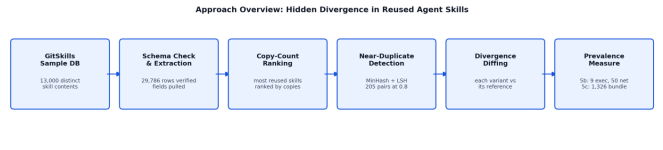
\includegraphics[width=\textwidth]{Images/approach_overview.png}
    \caption{Approach overview}
    \label{fig:approach_overview}
\end{figure*}

We worked with the data from the GitSkills sample on GitHub from the Destefanis et al. paper, which has 29,786 skill file rows, 13,000 distinct contents, with content fetched for 13,016 rows. We decided to use the sample because the full release is 44 gigabytes, too large for a preliminary analysis. The sample has the same structure as the full release, so it is enough to run the pipeline and produce pilot numbers. Our analysis code is available at \url{https://github.com/FrillySnake/ssw625_project}, and the GitSkills dataset is available at \url{https://doi.org/10.5281/zenodo.21875637} [1].

\subsection{Schema Check \& Extraction}
The first script "inspect" opened the database and listed its tables. It then ran count checks and every number matched: 29,786 rows and 13,000 distinct contents. It then pulls file\_sha, repo name, path, and content for each skill, and the content\_fetched check showed 13,016 rows actually have 
text to analyze.

\subsection{Copy-Count Ranking}
The second script groups every skill file by its file\_sha and counts how many copies each distinct skill has. It ranks them, and the ranking shows that skill reuse is concentrated. 9,622 of the 13,000 skills are copied exactly once, while 13 are copied over 100 times. The most copied skill sits at 188 copies, which gives you the short list of widely reused skills the rest of the pipeline investigates. 

\subsection{Near-Duplicate Detection}
From the Destefanis et al. paper, we know that exact hash matching only catches byte identical copies, so a skill that was copied and then edited slips through. In order to catch those, we normalized each skill text and broke it into overlapping 5 word shingles. We then hashed the shingle sets with MinHash at 128 permutations and used LSH at a 0.8 threshold to find candidate pairs without comparing all 84 million pairs. We verified each candidate with exact Jaccard and kept the pairs at or above 0.8 with different hashes, which gave 205 near duplicate pairs. Figure~\ref{fig:whitebox} shows this pipeline in white-box form, including the divergence diffing of Section 4.4.

\subsection{Divergence Diffing}
Script 04, "divergence", diffs each of the 205 pairs line by line against its reference, flagging lines present in one side but not the other. We then check those new lines against two fixed token lists: command execution with curl, wget, chmod +x, eval, exec, subprocess, os.system, and network 
access with http, https, fetch, requests. This is a heuristic flag, not proof of intent, but it surfaces exactly the pattern our paper warns about: a quiet download or shell command tucked into a copied skill.

\begin{figure*}[t]
\centering
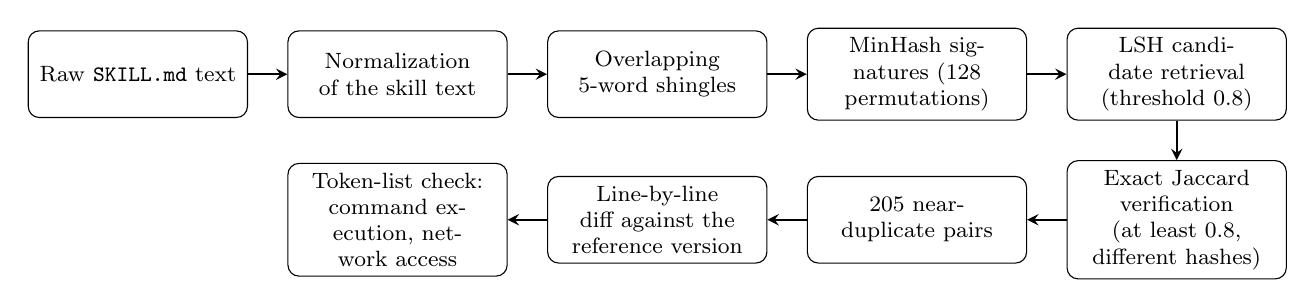
\begin{tikzpicture}[
  box/.style={draw, rounded corners, align=center, font=\footnotesize, minimum height=1.1cm, text width=2.55cm},
  arrow/.style={->, >=stealth, thick},
  node distance=0.5cm]
\node[box] (raw) {Raw \texttt{SKILL.md} text};
\node[box, right=of raw] (norm) {Normalization of the skill text};
\node[box, right=of norm] (shingle) {Overlapping 5-word shingles};
\node[box, right=of shingle] (minhash) {MinHash signatures (128 permutations)};
\node[box, right=of minhash] (lsh) {LSH candidate retrieval (threshold 0.8)};
\node[box, below=of lsh] (jac) {Exact Jaccard verification (at least 0.8, different hashes)};
\node[box, left=of jac] (pairs) {205 near-duplicate pairs};
\node[box, left=of pairs] (diff) {Line-by-line diff against the reference version};
\node[box, left=of diff] (tokens) {Token-list check: command execution, network access};
\draw[arrow] (raw) -- (norm);
\draw[arrow] (norm) -- (shingle);
\draw[arrow] (shingle) -- (minhash);
\draw[arrow] (minhash) -- (lsh);
\draw[arrow] (lsh) -- (jac);
\draw[arrow] (jac) -- (pairs);
\draw[arrow] (pairs) -- (diff);
\draw[arrow] (diff) -- (tokens);
\end{tikzpicture}
\caption{White-box view of the near-duplicate pipeline: how skill text is pre-processed (normalization, overlapping 5-word shingles) and represented (MinHash signatures) before candidate pairs are retrieved with LSH, verified with exact Jaccard, and diffed line by line against the token lists.}
\label{fig:whitebox}
\end{figure*}

\subsection{Prevalence Measure}
The final measure is the share of near duplicate pairs where one side adds a risky capability, 6 of 205 pairs with new command execution and 16 of 205 with new network access. Separately, 2 of the 13,000 distinct skills bundle executable files, although these skills do not have any reach and are limited to their corresponding repositories due to the limited size of the sample.

\subsection{Manual Analysis of the Dataset} 
We opened the sample database and read through a few of the most copied skills by hand, including their front matter and folder contents. We then looked at the artifact\_siblings table to see what files travel alongside the skill folders, and checked which skills carry scripts or reference documents. 

Finally we compared a few copies of the same content across different repositories to see how much they vary. 

The manual look showed us that copies of the same content are often not byte identical, small edits, reworded descriptions, extra lines, which is why exact hashing alone misses them. Also a noticeable share of the widely copied skills bundled scripts or reference files, and some variants added download commands that the original never had. The differences between copies were usually small and tucked away, which confirmed that a line level diff was the right way to catch them. The manual analysis therefore set the design. We ranked by copies first so the pipeline spends its effort on the widely reused skills where drift matters most. We then used near duplicate detection to recover the edited copies, then a line level diff with fixed token lists so the measurement is reproducible and anyone can rerun it. The result is reported as a prevalence share: how often copied skills contain hidden divergence, and what type of risky capability was introduced. 

\section{Experimental Results}
\label{Section:Result}
\begin{figure*}[t]
    \centering
    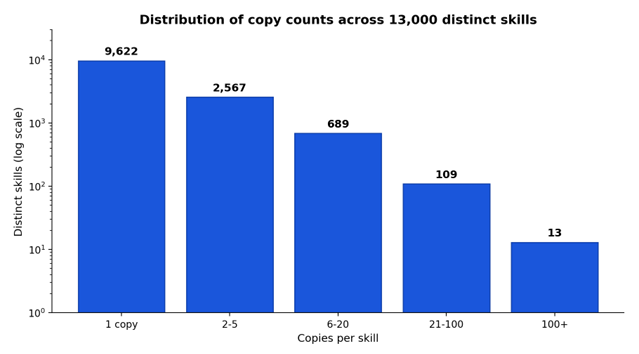
\includegraphics[width=\textwidth]{Images/results1.png}
    \caption{Distribution of copy counts across the 13,000 distinct skills in the sample. The y axis is a logarithmic scale.}
    \label{fig:results1}
\end{figure*}

\subsection{RQ 5b — Modified copies introducing new capabilities}
\begin{center}
    Question: Do modified copies of widely reused skills introduce command execution or 
network access absent from the original? 
\end{center}

To find modified copies, we ran MinHash plus LSH at 0.8 Jaccard on normalized text broken into 5 word shingles, which produced 205 near duplicate pairs. Then for each pair we diffed the two texts line by line in both directions. A pair counted as a hit when a line present in one side carried a command execution or network access token that the other side did not have. We found that 6 of the 205 pairs added command execution on one side, and 16 of 205 pairs added network access on one side, most often an https URL or a curl download. This means that roughly 7.8\% modified copies of a reused skill quietly gains a capability the original did not have, which is the supply chain pattern showing up in real data.

\subsection{RQ 5c — Bundled executables and their reach}
\begin{center}
    Question: How often do skills bundle executable files, and how widely are these skills 
copied? 
\end{center}

To measure bundling, we used a similar heuristic-based approach. Combining \texttt{artifacts} with \texttt{artifact\_siblings}, we search for skills with sibling entry names that correspond to a matching identifier token indicating an executable file (e.g. \texttt{.exe}, \texttt{.bin}, etc.), with the number of distinct repositories across which such a skill can be found being its reach. \\ 
We found that 2 of 13,000 distinct skills bundle executable files, though, due to the limited size of the sample, there is not much evidence of these skills having reach beyond their own repositories.

\subsection{Examples of Important Results}
Our experiments are not perfect; they produce numerous false positives and false negatives. For example, consider one of the two skills returned from the executable bundling algorithm. It corresponds to an element in \texttt{artifact\_siblings} with \\ \texttt{entry\_sha}=2707ee963ff1d0328929efd5a46ed66d23c7c86c. This file contains the \texttt{.bin} extension in a few lines, clearly not intending a malicious hack but rather an innocent download.

\begin{lstlisting}[language=Python, caption=False Positive Code]
pip install esptool mpremote
# get ESP32_GENERIC_S3 (SPIRAM / octal variant) .bin from micropython.org/download
esptool --chip esp32s3 --port <PORT> erase_flash
esptool --chip esp32s3 --port <PORT> --baud 460800 write_flash -z 0x0 ESP32_GENERIC_S3-*.bin
\end{lstlisting}

Unfortunately, the sample's limited size and variety of content does not leave any false negatives or true positives to analyze comprehensively.


\section{Discussion}
\label{Section:Discussion}

Our findings demonstrate that copy-based reuse in AI agent skill ecosystems introduces a potential supply-chain risk that cannot be identified through exact hash matching alone. While exact copies account for a significant portion of the GitSkills dataset, modified copies are particularly interesting from a security perspective. A skill may retain almost all of its original instructions while introducing a small change that alters how an AI agent interacts with the system. These changes may be difficult to notice during manual review, especially when the modified skill closely resembles a familiar or widely reused version.

The distribution of copy counts also highlights the importance of focusing on frequently reused skills. Of the 13,000 distinct contents analyzed, 9,622 appear only once, while 13 appear more than 100 times. The most frequently copied skill appears 188 times. This concentration suggests that a relatively small number of skills account for a substantial amount of reuse. Consequently, a malicious modification introduced into a popular skill could potentially affect multiple repositories if subsequent developers adopt the modified version. However, our dataset does not establish that such propagation has occurred.

Our near-duplicate detection pipeline identified 205 pairs of skills with different content hashes but a Jaccard similarity of at least 0.8. Among these pairs, 6 (2.9\%) contained differences in command execution tokens, while 16 (7.8\%) contained differences in network access tokens. These categories are not necessarily mutually exclusive, and the results should therefore be interpreted separately rather than added together. More importantly, the presence of these tokens does not establish malicious intent. A newly introduced URL, for example, may simply reference documentation, while a shell command may be necessary for legitimate functionality.

Nevertheless, the results illustrate how capabilities associated with potentially dangerous behavior can appear within otherwise similar skill files. This is particularly relevant to AI agents because \texttt{SKILL.md} files contain natural-language instructions that may influence an agent's actions. Unlike conventional software dependencies, these instructions do not necessarily pass through compilation or other traditional verification mechanisms before being interpreted by an agent. As a result, seemingly minor modifications may have consequences beyond their apparent size.

The executable bundling experiment further demonstrates the limitations of relying on file extensions and structural indicators. Only 2 of the 13,000 distinct skills were flagged as containing potential executable files, and neither demonstrated substantial reach within the sample. However, our manual inspection revealed that at least one flagged example involved legitimate MicroPython firmware instructions rather than evidence of malicious behavior. This illustrates the difficulty of distinguishing actual security threats from ordinary development functionality using simple heuristics.

Taken together, these findings suggest that near-duplicate detection is better suited as an initial screening mechanism than as a standalone malware detector. The combination of MinHash, LSH, and divergence analysis can reduce the number of files requiring examination and highlight modifications that deserve additional attention. Such an approach could complement existing security scanners by identifying suspicious differences between related skills rather than attempting to classify each skill independently.

This distinction is important when comparing our work to existing research. Previous studies have examined malicious skills, prompt injection, and manipulation of skill discovery mechanisms [2, 3, 4]. Our study instead focuses on the structural relationship between reused skills and the introduction of potentially risky capabilities. While the results do not establish the prevalence of malicious modifications, they provide preliminary evidence that capability-related divergence can be detected through a reproducible analysis of publicly available skill files.

\section{Threats To Validity}
\label{Section:Threats}

\subsection{Conclusion Validity}

This study suffers most strongly from threats to its conclusion validity. Three main avenues were identified and explored for attackers to introduce potentially malicious behavior: command execution, network access, and bundled executable files. However, the presence of these capabilities does not necessarily indicate malicious intent. Many legitimate skills require external resources, shell commands, or executable dependencies to perform their intended tasks.

Therefore, the 6 pairs flagged for command execution and the 16 pairs flagged for network access should not be interpreted as confirmed supply-chain attacks. They represent detected differences in capability-related tokens between highly similar files. The two categories may also overlap, meaning that their counts cannot be combined to calculate an overall prevalence without examining the intersection.

Furthermore, the study does not establish a ground-truth classification of benign and malicious skills. Without such a classification, we cannot reliably measure precision, recall, or false-positive and false-negative rates. Although manual inspection identified an example of a false positive in the executable bundling experiment, it was not sufficiently comprehensive to validate every flagged result.

Ultimately, our conclusions are limited to the prevalence of detectable capability-related divergence within the analyzed sample. The results support the existence of potentially security-relevant modifications, but do not establish how frequently those modifications represent actual attacks.

\subsection{Internal Validity}

Another issue is inherent to the heuristic-based approaches utilized throughout our study. Heuristics are imperfect and cannot account for every possible implementation of command execution, network access, or executable bundling.

For example, executable files may use extensions other than those included in our search, or may have no extension at all. Similarly, our divergence analysis relies on a fixed collection of command execution and network access patterns. A modified skill could introduce equivalent functionality using different syntax, indirect references, or instructions expressed entirely in natural language without triggering any of the selected patterns.

The near-duplicate detection process introduces additional limitations. Our implementation uses normalized text, overlapping 5-word shingles, MinHash signatures with 128 permutations, and LSH with a threshold of 0.8. Although candidate pairs are subsequently verified using exact Jaccard similarity, LSH is a probabilistic retrieval method and may fail to retrieve some genuinely similar files. Consequently, the 205 detected pairs should not be assumed to represent every near-duplicate relationship in the sample.

Additionally, the divergence script compares the presence of token categories across the complete contents of each skill. It does not verify whether a matching token occurs specifically within an added line, nor does it determine which version of a skill was created first. Therefore, describing a difference as an introduced capability does not establish the historical direction of the modification.

These limitations may influence both the number of detected pairs and the classification of capability differences. However, the fixed thresholds and detection patterns make the analysis reproducible and allow future experiments to evaluate the effect of alternative configurations.

\subsection{Construct Validity}

Our capability measures are token-based, meaning that they capture the presence of particular expressions rather than verified executable behavior. For instance, the appearance of an HTTPS URL does not necessarily demonstrate network access, and a reference to a command does not establish that an agent will execute it. Conversely, an instruction directing an agent to perform a dangerous action may contain none of the patterns included in our detection lists.

Similarly, textual similarity is not equivalent to behavioral similarity. Two skills may share nearly identical wording while instructing agents to behave differently, whereas two skills with different wording may perform the same task. Our use of 5-word shingles and Jaccard similarity captures lexical overlap but does not account for the meaning or execution of the instructions.

Very short skills also produce relatively few shingles, making their similarity measurements less informative. Furthermore, only records with successfully fetched content could be included in the textual analysis. The resulting measurements therefore describe the subset of skills accessible through the sample database rather than all records represented in the dataset.

The executable bundling measure presents a related concern. File extensions provide only an approximation of executable content and do not establish that an executable is malicious, reachable, or invoked by a skill. The MicroPython example identified during manual inspection illustrates this limitation.

Consequently, the constructs measured in this study should be understood as textual similarity, capability-related token divergence, and potential executable bundling rather than direct measurements of malicious behavior.

\subsection{External Validity}

We worked with the GitSkills sample rather than the complete dataset because the full release is approximately 44 gigabytes, making it impractical for our preliminary analysis. Although the sample follows the same database structure as the complete release, this does not guarantee that it preserves the same distribution of skills, modifications, or security-relevant characteristics.

The sample contains 29,786 skill file records, of which 13,016 have fetched content available for analysis. As a result, our findings may not generalize to skills whose contents were unavailable or to the millions of additional files in the complete dataset.

Furthermore, the executable bundling experiment identified only two distinct skills with potential executable files, neither showing meaningful reuse beyond its corresponding repository within the sample. This limited observation cannot establish the prevalence or reach of bundled executables throughout the broader ecosystem.

Finally, GitSkills focuses on public GitHub repositories. Skills distributed through dedicated registries, private repositories, or other hosting platforms may exhibit different reuse patterns and security characteristics. The findings should therefore be treated as preliminary measurements of one publicly available dataset rather than representative estimates for all AI agent skill ecosystems.

\section{Conclusion}
\label{Section:Conclusion}

This paper investigated the potential supply-chain risks associated with copy-based reuse of AI agent skills, focusing on how small modifications to \texttt{SKILL.md} files may introduce capabilities absent from otherwise similar versions. Using the GitSkills sample dataset, we developed a reproducible pipeline combining copy-count ranking, near-duplicate detection, divergence analysis, and executable bundling checks.

Our analysis confirmed that skill reuse is concentrated among a relatively small number of popular files. Using MinHash and LSH followed by exact Jaccard verification, we identified 205 near-duplicate pairs with different content hashes and at least 0.8 similarity. Of these pairs, 6 exhibited differences in command execution tokens and 16 exhibited differences in network access tokens. Separately, the executable bundling analysis flagged 2 of the 13,000 distinct skills, although manual inspection demonstrated that such detections may correspond to legitimate functionality.

These results illustrate both the usefulness and limitations of structural analysis. While exact hashing can identify identical copies, it cannot reveal modifications introduced into reused skills. Near-duplicate detection helps address this limitation by identifying closely related files and exposing their differences. However, our experiments also demonstrate that detecting potentially risky capabilities is not equivalent to identifying malicious behavior.

The main contribution of this study is therefore not a definitive malware detection system, but a practical method for identifying capability-related divergence in reused AI agent skills. As agent ecosystems continue to expand, understanding how instructions and associated files are copied, modified, and redistributed will become increasingly important. Our findings suggest that examining relationships between skill versions can provide useful information for software supply-chain security and establish a foundation for more comprehensive analysis.

\section{Future Work}
\label{Section:FutureWork}

The most immediate extension of this research would be to apply the pipeline to the complete GitSkills dataset. Our current experiments use only the publicly available sample, which limits the number and variety of skills that can be analyzed. Expanding the analysis to all 3,797,117 records would provide a stronger basis for estimating the prevalence of capability-related divergence and examining whether the patterns identified in this study persist at a larger scale.

Another important improvement would be to refine the detection heuristics. The current implementation searches for a relatively small set of command execution and network access patterns, making it susceptible to both false positives and false negatives. Future work could incorporate syntax-aware analysis, more comprehensive command patterns, and improved inspection of associated files. In particular, detecting executable content through file signatures rather than extensions alone would provide a more reliable measure of bundled executable files.

We would also like to explore semantic analysis as an alternative to purely lexical comparison. Our current approach identifies near-duplicates through overlapping word shingles, which works well for small textual changes but may miss modifications expressed through substantial rewording. Embedding-based similarity or language-model-assisted analysis could help identify skills that retain the same purpose while introducing new instructions. Such methods could also help distinguish ordinary documentation changes from modifications that alter an agent's expected behavior.

A further direction involves establishing a manually labeled evaluation dataset. By reviewing a representative set of flagged and unflagged skills, future experiments could classify modifications as benign, suspicious, or malicious according to predefined criteria. This would make it possible to calculate precision, recall, and false-positive rates, providing a clearer assessment of the effectiveness of each detection method.

Future research could also investigate the historical propagation of modified skills across repositories. Our current analysis identifies similarities and differences but does not establish which version appeared first or whether one repository directly copied another. Incorporating commit histories, timestamps, and repository relationships could help reconstruct the evolution of skill variants and determine whether potentially dangerous modifications spread beyond their original source.

Finally, the pipeline could be extended into a practical security tool for developers and AI agent operators. Rather than relying exclusively on scanning individual skills, such a tool could compare newly imported skills against known versions and flag unexpected changes in command execution, network access, or bundled files. This would allow developers to review potentially significant modifications before incorporating externally sourced skills into their agents.

Together, these improvements would move the project beyond preliminary structural measurements toward a more reliable and scalable approach for detecting and understanding supply-chain risks in AI agent skill ecosystems.


\begin{thebibliography}{4}
\bibitem{destefanis} G. Destefanis, D. Graziotin, M. Vaccargiu, and M. Ortu, “GitSkills: A Dataset of Agent Skills on GitHub,” arXiv:2608.10906, 2026. Dataset: https://doi.org/10.5281/zenodo.21875637
\bibitem{owasp} OWASP Foundation, “AST01: Malicious Skills,” OWASP Agentic Skills Top 10, 2026. [Online]. Available: https://owasp.github.io/www-project-agentic-skills-top-10/ast01. (accessed: Sep. 29, 2026).
\bibitem{beurerkellner} L. Beurer-Kellner, A. Kudrinskii, M. Milanta, K. B. Nielsen, H. Sarkar, and L. Tal, “Snyk Finds Prompt Injection in 36\%, 1467 Malicious Payloads in a ToxicSkills Study of Agent Skills Supply Chain Compromise,” Snyk, Feb. 5, 2026. [Online]. Available: https://snyk.io/blog/toxicskills-malicious-ai-agent-skills-clawhub/. [Accessed: Sep. 29, 2026].
\bibitem{saha} S. Saha, K. Faghih, S. Feizi, “Under the Hood of SKILL.md: Semantic Supply-chain Attacks on AI Agent Skill Registry” 2026. [Online]. Available: arXiv:2605.11418.
\end{thebibliography}

\end{document}
\endinput
%%
%% End of file `sample-authordraft.tex'.
